\documentclass[]{report}
\usepackage{tikz}
\usepackage{listings}
\usepackage{color}

\definecolor{dkgreen}{rgb}{0,0.6,0}
\definecolor{gray}{rgb}{0.5,0.5,0.5}
\definecolor{mauve}{rgb}{0.58,0,0.82}
%opening
\title{SY19}
\author{}

\begin{document}
	
\lstset{frame=tb,
	language=R,
	aboveskip=3mm,
	belowskip=3mm,
	showstringspaces=false,
	columns=flexible,
	basicstyle={\small\ttfamily},
	numbers=none,
	numberstyle=\tiny\color{gray},
	keywordstyle=\color{blue},
	commentstyle=\color{dkgreen},
	stringstyle=\color{mauve},
	breaklines=true,
	breakatwhitespace=true,
	tabsize=3
}

\maketitle

\part{Abreviations}
	

\begin{abstract}

\end{abstract}

\part{Introduction}

\part{Ex 1}

\part{Ex 2 - Breast Cancer Recurring Time}

\section{Introduction}
This part aims to build the best model to predict the recurring time of breast cancer based on about 30 features computed from a breast mass.  This regression problem will take advantage of a given dataset describing about 200 patient cases.

\section{Dataset Description}
We first take a look at the original dataset to get first hints on how each feature contributes to the recurring time.

The dataset comprises 194 patient cases, each of which is described through 32 features and the cancer recurring time \texttt{Time}.

\subsection{Time}

\subsection{Features Description}

\subsubsection{Feature Correlation}
Based on the definition of the parameters, we already know that many features are correlated :
\begin{itemize}
	\item The mean of each parameters is bigger than the "worst" value;
	\item The radius, the perimeter and the area are linked together;
	\item The compactness can be computed with the perimeter and the area thanks to the given formula : $Compactness = \frac{perimeter^2}{area - 1}$
	\item *MORE FEATURE CORRELATION*
\end{itemize}

\subsection{Data Relevance}
We should first check that every point is relevant to our study, in other words, that there is no abnormal point in the dataset. Cook's Distance is an interesting measure to verify this important criteria, it can be computed after a simple Linear Regression.

*TALK ABOUT COOK'S DISTANCE*

According to this graph, no point is located beyond the critical Cook's boundary. This means that we can potentially use each and every patient case of our dataset to build our regression model. 

\subsection{Relation between "feature" and "time"}
*GRAPH : each Feature vs. Time*

*QQ-PLOT : Non Linearities*

*Heteroscedasticity*


\section{Measures to Compare Models}
Before building any model, we have to properly define the measures we will later use to compare them. 

\subsection{Some Measures}
*TALK ABOUT MSE, R2 AND OTHER STUFF*

\subsection{Data Split}
These measures should not be applied on a set whose data was also used to train the model. Indeed, this would include a biais that might distort our conclusions. To cope with this problem, we have to split the dataset into two disjointed sets : 
\begin{itemize}
	\item Training Set : About 75\% of the dataset dedicated to the building the model;
	\item Test Set : The remaining 25\% only used at the end to provide some kind of objective measure of the model performance.
\end{itemize} 

Once it is done, we can finally dive in the model building.

\section{K-nearest neighbors (KNN)}
\subsection{Idea}
We start our analysis with a very simple model called the KNN.
Given an positive integer k and a test observation x0. The KNN model first identifies the k closest points to x0 from the training data. Then estimates \\ 

The KNN model in R is done by calling the function reg of the package knn. As we will see in the following sections, For most prediction algorithms, we first have to build the prediction model on the training data, and then use the model to test our predictions. However, the KNN function does both in a single step.\\ 
In order to find the best k we set a maximum number of neighbors to be considered (in our model it is 20), then we calculate the MSE for each k which is the mean of the squared difference between the real value of Time and the predicted one. All the steps are detailed in the code below.\\

\begin{lstlisting}
library(FNN)
library(tikzDevice)
k_max = 120;
MSE = rep(0,k_max)

for( k in 1:k_max)
{
reg = knn.reg(train=cancer.train.x, test=cancer.test.x, y=cancer.train.y, k=k)
MSE[k] = mean((cancer.test.y - reg$pred)^2)
}

best_k_test = which.min(MSE)
best_k_mse = MSE[best_k_test]
sprintf("Best knn1 = %d and the best MSE1 = %f", best_k_test, best_k_mse)

tikz('Figures/knn.tex',width=5, height=5)

plot(1:k_max, MSE, xlab='k', ylab='MSE', main='MSE against k neighbours')
points(x = best_k_test, y = best_k_mse, col = "red", pch = 16)
abline(h = best_k_mse, col='red')
abline(v = best_k_test, col='red')
dev.off()
\end{lstlisting}

The graph below shows the MSE plotted against the values of k in a range from 1 to 20. We can notice that a minimum is reached between 10 and 20. We use the function which.min that returns the index of the minimum value.\\
	
\begin{figure}[!hb]
	\centering
	% Created by tikzDevice version 0.10.1 on 2016-11-04 23:52:30
% !TEX encoding = UTF-8 Unicode
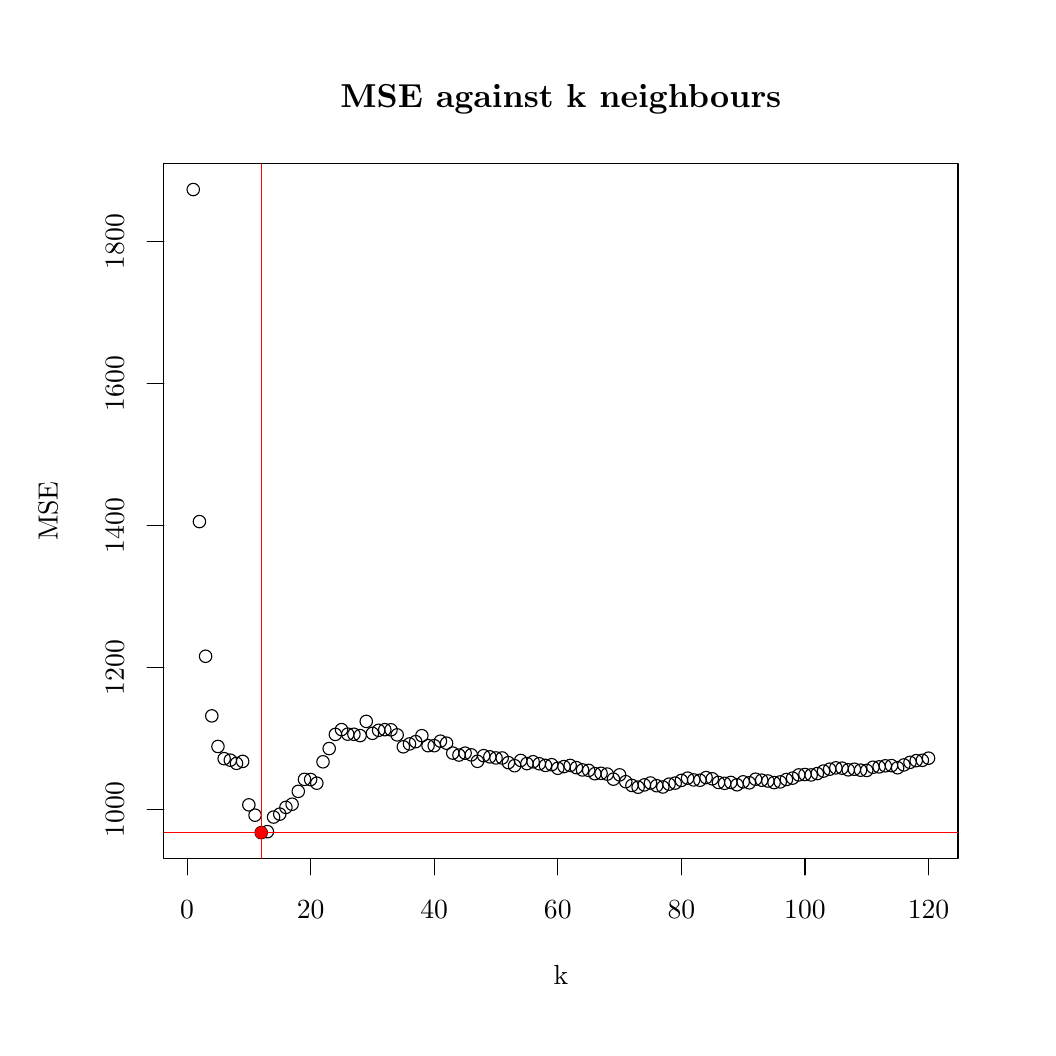
\begin{tikzpicture}[x=1pt,y=1pt]
\definecolor{fillColor}{RGB}{255,255,255}
\path[use as bounding box,fill=fillColor,fill opacity=0.00] (0,0) rectangle (361.35,361.35);
\begin{scope}
\path[clip] ( 49.20, 61.20) rectangle (336.15,312.15);
\definecolor{drawColor}{RGB}{0,0,0}

\path[draw=drawColor,line width= 0.4pt,line join=round,line cap=round] ( 59.83,302.86) circle (  2.25);

\path[draw=drawColor,line width= 0.4pt,line join=round,line cap=round] ( 62.06,182.87) circle (  2.25);

\path[draw=drawColor,line width= 0.4pt,line join=round,line cap=round] ( 64.29,134.21) circle (  2.25);

\path[draw=drawColor,line width= 0.4pt,line join=round,line cap=round] ( 66.53,112.66) circle (  2.25);

\path[draw=drawColor,line width= 0.4pt,line join=round,line cap=round] ( 68.76,101.61) circle (  2.25);

\path[draw=drawColor,line width= 0.4pt,line join=round,line cap=round] ( 70.99, 97.20) circle (  2.25);

\path[draw=drawColor,line width= 0.4pt,line join=round,line cap=round] ( 73.22, 96.66) circle (  2.25);

\path[draw=drawColor,line width= 0.4pt,line join=round,line cap=round] ( 75.46, 95.51) circle (  2.25);

\path[draw=drawColor,line width= 0.4pt,line join=round,line cap=round] ( 77.69, 96.22) circle (  2.25);

\path[draw=drawColor,line width= 0.4pt,line join=round,line cap=round] ( 79.92, 80.51) circle (  2.25);

\path[draw=drawColor,line width= 0.4pt,line join=round,line cap=round] ( 82.16, 76.78) circle (  2.25);

\path[draw=drawColor,line width= 0.4pt,line join=round,line cap=round] ( 84.39, 70.49) circle (  2.25);

\path[draw=drawColor,line width= 0.4pt,line join=round,line cap=round] ( 86.62, 70.83) circle (  2.25);

\path[draw=drawColor,line width= 0.4pt,line join=round,line cap=round] ( 88.85, 76.10) circle (  2.25);

\path[draw=drawColor,line width= 0.4pt,line join=round,line cap=round] ( 91.09, 77.16) circle (  2.25);

\path[draw=drawColor,line width= 0.4pt,line join=round,line cap=round] ( 93.32, 79.60) circle (  2.25);

\path[draw=drawColor,line width= 0.4pt,line join=round,line cap=round] ( 95.55, 80.74) circle (  2.25);

\path[draw=drawColor,line width= 0.4pt,line join=round,line cap=round] ( 97.78, 85.39) circle (  2.25);

\path[draw=drawColor,line width= 0.4pt,line join=round,line cap=round] (100.02, 89.73) circle (  2.25);

\path[draw=drawColor,line width= 0.4pt,line join=round,line cap=round] (102.25, 89.67) circle (  2.25);

\path[draw=drawColor,line width= 0.4pt,line join=round,line cap=round] (104.48, 88.34) circle (  2.25);

\path[draw=drawColor,line width= 0.4pt,line join=round,line cap=round] (106.72, 96.07) circle (  2.25);

\path[draw=drawColor,line width= 0.4pt,line join=round,line cap=round] (108.95,100.86) circle (  2.25);

\path[draw=drawColor,line width= 0.4pt,line join=round,line cap=round] (111.18,105.97) circle (  2.25);

\path[draw=drawColor,line width= 0.4pt,line join=round,line cap=round] (113.41,107.71) circle (  2.25);

\path[draw=drawColor,line width= 0.4pt,line join=round,line cap=round] (115.65,106.06) circle (  2.25);

\path[draw=drawColor,line width= 0.4pt,line join=round,line cap=round] (117.88,106.02) circle (  2.25);

\path[draw=drawColor,line width= 0.4pt,line join=round,line cap=round] (120.11,105.55) circle (  2.25);

\path[draw=drawColor,line width= 0.4pt,line join=round,line cap=round] (122.34,110.67) circle (  2.25);

\path[draw=drawColor,line width= 0.4pt,line join=round,line cap=round] (124.58,106.36) circle (  2.25);

\path[draw=drawColor,line width= 0.4pt,line join=round,line cap=round] (126.81,107.45) circle (  2.25);

\path[draw=drawColor,line width= 0.4pt,line join=round,line cap=round] (129.04,107.68) circle (  2.25);

\path[draw=drawColor,line width= 0.4pt,line join=round,line cap=round] (131.28,107.63) circle (  2.25);

\path[draw=drawColor,line width= 0.4pt,line join=round,line cap=round] (133.51,105.80) circle (  2.25);

\path[draw=drawColor,line width= 0.4pt,line join=round,line cap=round] (135.74,101.49) circle (  2.25);

\path[draw=drawColor,line width= 0.4pt,line join=round,line cap=round] (137.97,102.52) circle (  2.25);

\path[draw=drawColor,line width= 0.4pt,line join=round,line cap=round] (140.21,103.35) circle (  2.25);

\path[draw=drawColor,line width= 0.4pt,line join=round,line cap=round] (142.44,105.51) circle (  2.25);

\path[draw=drawColor,line width= 0.4pt,line join=round,line cap=round] (144.67,101.90) circle (  2.25);

\path[draw=drawColor,line width= 0.4pt,line join=round,line cap=round] (146.90,101.89) circle (  2.25);

\path[draw=drawColor,line width= 0.4pt,line join=round,line cap=round] (149.14,103.53) circle (  2.25);

\path[draw=drawColor,line width= 0.4pt,line join=round,line cap=round] (151.37,102.80) circle (  2.25);

\path[draw=drawColor,line width= 0.4pt,line join=round,line cap=round] (153.60, 99.22) circle (  2.25);

\path[draw=drawColor,line width= 0.4pt,line join=round,line cap=round] (155.84, 98.52) circle (  2.25);

\path[draw=drawColor,line width= 0.4pt,line join=round,line cap=round] (158.07, 99.20) circle (  2.25);

\path[draw=drawColor,line width= 0.4pt,line join=round,line cap=round] (160.30, 98.58) circle (  2.25);

\path[draw=drawColor,line width= 0.4pt,line join=round,line cap=round] (162.53, 96.25) circle (  2.25);

\path[draw=drawColor,line width= 0.4pt,line join=round,line cap=round] (164.77, 98.28) circle (  2.25);

\path[draw=drawColor,line width= 0.4pt,line join=round,line cap=round] (167.00, 97.86) circle (  2.25);

\path[draw=drawColor,line width= 0.4pt,line join=round,line cap=round] (169.23, 97.46) circle (  2.25);

\path[draw=drawColor,line width= 0.4pt,line join=round,line cap=round] (171.46, 97.45) circle (  2.25);

\path[draw=drawColor,line width= 0.4pt,line join=round,line cap=round] (173.70, 95.77) circle (  2.25);

\path[draw=drawColor,line width= 0.4pt,line join=round,line cap=round] (175.93, 94.66) circle (  2.25);

\path[draw=drawColor,line width= 0.4pt,line join=round,line cap=round] (178.16, 96.56) circle (  2.25);

\path[draw=drawColor,line width= 0.4pt,line join=round,line cap=round] (180.40, 95.42) circle (  2.25);

\path[draw=drawColor,line width= 0.4pt,line join=round,line cap=round] (182.63, 96.09) circle (  2.25);

\path[draw=drawColor,line width= 0.4pt,line join=round,line cap=round] (184.86, 95.37) circle (  2.25);

\path[draw=drawColor,line width= 0.4pt,line join=round,line cap=round] (187.09, 94.77) circle (  2.25);

\path[draw=drawColor,line width= 0.4pt,line join=round,line cap=round] (189.33, 95.02) circle (  2.25);

\path[draw=drawColor,line width= 0.4pt,line join=round,line cap=round] (191.56, 93.74) circle (  2.25);

\path[draw=drawColor,line width= 0.4pt,line join=round,line cap=round] (193.79, 94.35) circle (  2.25);

\path[draw=drawColor,line width= 0.4pt,line join=round,line cap=round] (196.02, 94.76) circle (  2.25);

\path[draw=drawColor,line width= 0.4pt,line join=round,line cap=round] (198.26, 93.96) circle (  2.25);

\path[draw=drawColor,line width= 0.4pt,line join=round,line cap=round] (200.49, 93.13) circle (  2.25);

\path[draw=drawColor,line width= 0.4pt,line join=round,line cap=round] (202.72, 92.97) circle (  2.25);

\path[draw=drawColor,line width= 0.4pt,line join=round,line cap=round] (204.95, 91.77) circle (  2.25);

\path[draw=drawColor,line width= 0.4pt,line join=round,line cap=round] (207.19, 91.91) circle (  2.25);

\path[draw=drawColor,line width= 0.4pt,line join=round,line cap=round] (209.42, 91.63) circle (  2.25);

\path[draw=drawColor,line width= 0.4pt,line join=round,line cap=round] (211.65, 89.80) circle (  2.25);

\path[draw=drawColor,line width= 0.4pt,line join=round,line cap=round] (213.89, 91.35) circle (  2.25);

\path[draw=drawColor,line width= 0.4pt,line join=round,line cap=round] (216.12, 88.88) circle (  2.25);

\path[draw=drawColor,line width= 0.4pt,line join=round,line cap=round] (218.35, 87.52) circle (  2.25);

\path[draw=drawColor,line width= 0.4pt,line join=round,line cap=round] (220.58, 86.89) circle (  2.25);

\path[draw=drawColor,line width= 0.4pt,line join=round,line cap=round] (222.82, 87.72) circle (  2.25);

\path[draw=drawColor,line width= 0.4pt,line join=round,line cap=round] (225.05, 88.41) circle (  2.25);

\path[draw=drawColor,line width= 0.4pt,line join=round,line cap=round] (227.28, 87.43) circle (  2.25);

\path[draw=drawColor,line width= 0.4pt,line join=round,line cap=round] (229.51, 86.97) circle (  2.25);

\path[draw=drawColor,line width= 0.4pt,line join=round,line cap=round] (231.75, 87.99) circle (  2.25);

\path[draw=drawColor,line width= 0.4pt,line join=round,line cap=round] (233.98, 88.38) circle (  2.25);

\path[draw=drawColor,line width= 0.4pt,line join=round,line cap=round] (236.21, 89.35) circle (  2.25);

\path[draw=drawColor,line width= 0.4pt,line join=round,line cap=round] (238.45, 90.17) circle (  2.25);

\path[draw=drawColor,line width= 0.4pt,line join=round,line cap=round] (240.68, 89.51) circle (  2.25);

\path[draw=drawColor,line width= 0.4pt,line join=round,line cap=round] (242.91, 89.41) circle (  2.25);

\path[draw=drawColor,line width= 0.4pt,line join=round,line cap=round] (245.14, 90.37) circle (  2.25);

\path[draw=drawColor,line width= 0.4pt,line join=round,line cap=round] (247.38, 89.92) circle (  2.25);

\path[draw=drawColor,line width= 0.4pt,line join=round,line cap=round] (249.61, 88.61) circle (  2.25);

\path[draw=drawColor,line width= 0.4pt,line join=round,line cap=round] (251.84, 88.29) circle (  2.25);

\path[draw=drawColor,line width= 0.4pt,line join=round,line cap=round] (254.07, 88.61) circle (  2.25);

\path[draw=drawColor,line width= 0.4pt,line join=round,line cap=round] (256.31, 87.77) circle (  2.25);

\path[draw=drawColor,line width= 0.4pt,line join=round,line cap=round] (258.54, 88.83) circle (  2.25);

\path[draw=drawColor,line width= 0.4pt,line join=round,line cap=round] (260.77, 88.49) circle (  2.25);

\path[draw=drawColor,line width= 0.4pt,line join=round,line cap=round] (263.01, 89.78) circle (  2.25);

\path[draw=drawColor,line width= 0.4pt,line join=round,line cap=round] (265.24, 89.43) circle (  2.25);

\path[draw=drawColor,line width= 0.4pt,line join=round,line cap=round] (267.47, 89.13) circle (  2.25);

\path[draw=drawColor,line width= 0.4pt,line join=round,line cap=round] (269.70, 88.57) circle (  2.25);

\path[draw=drawColor,line width= 0.4pt,line join=round,line cap=round] (271.94, 88.81) circle (  2.25);

\path[draw=drawColor,line width= 0.4pt,line join=round,line cap=round] (274.17, 89.68) circle (  2.25);

\path[draw=drawColor,line width= 0.4pt,line join=round,line cap=round] (276.40, 90.17) circle (  2.25);

\path[draw=drawColor,line width= 0.4pt,line join=round,line cap=round] (278.63, 91.33) circle (  2.25);

\path[draw=drawColor,line width= 0.4pt,line join=round,line cap=round] (280.87, 91.48) circle (  2.25);

\path[draw=drawColor,line width= 0.4pt,line join=round,line cap=round] (283.10, 91.33) circle (  2.25);

\path[draw=drawColor,line width= 0.4pt,line join=round,line cap=round] (285.33, 91.82) circle (  2.25);

\path[draw=drawColor,line width= 0.4pt,line join=round,line cap=round] (287.57, 92.72) circle (  2.25);

\path[draw=drawColor,line width= 0.4pt,line join=round,line cap=round] (289.80, 93.40) circle (  2.25);

\path[draw=drawColor,line width= 0.4pt,line join=round,line cap=round] (292.03, 93.88) circle (  2.25);

\path[draw=drawColor,line width= 0.4pt,line join=round,line cap=round] (294.26, 93.78) circle (  2.25);

\path[draw=drawColor,line width= 0.4pt,line join=round,line cap=round] (296.50, 93.17) circle (  2.25);

\path[draw=drawColor,line width= 0.4pt,line join=round,line cap=round] (298.73, 93.39) circle (  2.25);

\path[draw=drawColor,line width= 0.4pt,line join=round,line cap=round] (300.96, 93.04) circle (  2.25);

\path[draw=drawColor,line width= 0.4pt,line join=round,line cap=round] (303.19, 92.95) circle (  2.25);

\path[draw=drawColor,line width= 0.4pt,line join=round,line cap=round] (305.43, 94.10) circle (  2.25);

\path[draw=drawColor,line width= 0.4pt,line join=round,line cap=round] (307.66, 94.23) circle (  2.25);

\path[draw=drawColor,line width= 0.4pt,line join=round,line cap=round] (309.89, 94.62) circle (  2.25);

\path[draw=drawColor,line width= 0.4pt,line join=round,line cap=round] (312.13, 94.70) circle (  2.25);

\path[draw=drawColor,line width= 0.4pt,line join=round,line cap=round] (314.36, 93.92) circle (  2.25);

\path[draw=drawColor,line width= 0.4pt,line join=round,line cap=round] (316.59, 94.94) circle (  2.25);

\path[draw=drawColor,line width= 0.4pt,line join=round,line cap=round] (318.82, 95.87) circle (  2.25);

\path[draw=drawColor,line width= 0.4pt,line join=round,line cap=round] (321.06, 96.49) circle (  2.25);

\path[draw=drawColor,line width= 0.4pt,line join=round,line cap=round] (323.29, 96.61) circle (  2.25);

\path[draw=drawColor,line width= 0.4pt,line join=round,line cap=round] (325.52, 97.38) circle (  2.25);
\end{scope}
\begin{scope}
\path[clip] (  0.00,  0.00) rectangle (361.35,361.35);
\definecolor{drawColor}{RGB}{0,0,0}

\path[draw=drawColor,line width= 0.4pt,line join=round,line cap=round] ( 57.60, 61.20) -- (325.52, 61.20);

\path[draw=drawColor,line width= 0.4pt,line join=round,line cap=round] ( 57.60, 61.20) -- ( 57.60, 55.20);

\path[draw=drawColor,line width= 0.4pt,line join=round,line cap=round] (102.25, 61.20) -- (102.25, 55.20);

\path[draw=drawColor,line width= 0.4pt,line join=round,line cap=round] (146.90, 61.20) -- (146.90, 55.20);

\path[draw=drawColor,line width= 0.4pt,line join=round,line cap=round] (191.56, 61.20) -- (191.56, 55.20);

\path[draw=drawColor,line width= 0.4pt,line join=round,line cap=round] (236.21, 61.20) -- (236.21, 55.20);

\path[draw=drawColor,line width= 0.4pt,line join=round,line cap=round] (280.87, 61.20) -- (280.87, 55.20);

\path[draw=drawColor,line width= 0.4pt,line join=round,line cap=round] (325.52, 61.20) -- (325.52, 55.20);

\node[text=drawColor,anchor=base,inner sep=0pt, outer sep=0pt, scale=  1.00] at ( 57.60, 39.60) {0};

\node[text=drawColor,anchor=base,inner sep=0pt, outer sep=0pt, scale=  1.00] at (102.25, 39.60) {20};

\node[text=drawColor,anchor=base,inner sep=0pt, outer sep=0pt, scale=  1.00] at (146.90, 39.60) {40};

\node[text=drawColor,anchor=base,inner sep=0pt, outer sep=0pt, scale=  1.00] at (191.56, 39.60) {60};

\node[text=drawColor,anchor=base,inner sep=0pt, outer sep=0pt, scale=  1.00] at (236.21, 39.60) {80};

\node[text=drawColor,anchor=base,inner sep=0pt, outer sep=0pt, scale=  1.00] at (280.87, 39.60) {100};

\node[text=drawColor,anchor=base,inner sep=0pt, outer sep=0pt, scale=  1.00] at (325.52, 39.60) {120};

\path[draw=drawColor,line width= 0.4pt,line join=round,line cap=round] ( 49.20, 78.86) -- ( 49.20,284.13);

\path[draw=drawColor,line width= 0.4pt,line join=round,line cap=round] ( 49.20, 78.86) -- ( 43.20, 78.86);

\path[draw=drawColor,line width= 0.4pt,line join=round,line cap=round] ( 49.20,130.18) -- ( 43.20,130.18);

\path[draw=drawColor,line width= 0.4pt,line join=round,line cap=round] ( 49.20,181.50) -- ( 43.20,181.50);

\path[draw=drawColor,line width= 0.4pt,line join=round,line cap=round] ( 49.20,232.81) -- ( 43.20,232.81);

\path[draw=drawColor,line width= 0.4pt,line join=round,line cap=round] ( 49.20,284.13) -- ( 43.20,284.13);

\node[text=drawColor,rotate= 90.00,anchor=base,inner sep=0pt, outer sep=0pt, scale=  1.00] at ( 34.80, 78.86) {1000};

\node[text=drawColor,rotate= 90.00,anchor=base,inner sep=0pt, outer sep=0pt, scale=  1.00] at ( 34.80,130.18) {1200};

\node[text=drawColor,rotate= 90.00,anchor=base,inner sep=0pt, outer sep=0pt, scale=  1.00] at ( 34.80,181.50) {1400};

\node[text=drawColor,rotate= 90.00,anchor=base,inner sep=0pt, outer sep=0pt, scale=  1.00] at ( 34.80,232.81) {1600};

\node[text=drawColor,rotate= 90.00,anchor=base,inner sep=0pt, outer sep=0pt, scale=  1.00] at ( 34.80,284.13) {1800};

\path[draw=drawColor,line width= 0.4pt,line join=round,line cap=round] ( 49.20, 61.20) --
	(336.15, 61.20) --
	(336.15,312.15) --
	( 49.20,312.15) --
	( 49.20, 61.20);
\end{scope}
\begin{scope}
\path[clip] (  0.00,  0.00) rectangle (361.35,361.35);
\definecolor{drawColor}{RGB}{0,0,0}

\node[text=drawColor,anchor=base,inner sep=0pt, outer sep=0pt, scale=  1.20] at (192.68,332.61) {\bfseries MSE against k neighbours};

\node[text=drawColor,anchor=base,inner sep=0pt, outer sep=0pt, scale=  1.00] at (192.68, 15.60) {k};

\node[text=drawColor,rotate= 90.00,anchor=base,inner sep=0pt, outer sep=0pt, scale=  1.00] at ( 10.80,186.67) {MSE};
\end{scope}
\begin{scope}
\path[clip] ( 49.20, 61.20) rectangle (336.15,312.15);
\definecolor{fillColor}{RGB}{255,0,0}

\path[fill=fillColor] ( 84.39, 70.49) circle (  2.25);
\definecolor{drawColor}{RGB}{255,0,0}

\path[draw=drawColor,line width= 0.4pt,line join=round,line cap=round] ( 49.20, 70.49) -- (336.15, 70.49);

\path[draw=drawColor,line width= 0.4pt,line join=round,line cap=round] ( 84.39, 61.20) -- ( 84.39,312.15);
\end{scope}
\end{tikzpicture}

	\caption{MSE against k neighbours}
\end{figure}

 The minimum MSE which yields to the best k is colored in red. Its coordinates correspond to (\textbf{12,967.386966}). The best k is therefore .
Now that we have the k that minimizes the MSE we call KNN algorithm with this best k and plot the predicted values against the real values. The figure above shows the result. The red line is the function y=x; so further are the points from this line the further are the predicted values ($\hat{y}$) from the real one (y).

\begin{lstlisting}
best_reg_test = knn.reg(train= cancer.train.x, test = cancer.test.x, y=cancer.train.y, k = best_k_test)
tikz('Figures/knn_predicted_test.tex',width=5, height=5)
plot(cancer.test.y, best_reg_test$pred, xlab='y', ylab='y-hat', main='y-hat (Predicted) against y')
abline(0,1, col='red')
dev.off() 
\end{lstlisting}

\begin{figure}[!h]
	\centering
	% Created by tikzDevice version 0.10.1 on 2016-11-04 23:52:30
% !TEX encoding = UTF-8 Unicode
\begin{tikzpicture}[x=1pt,y=1pt]
\definecolor{fillColor}{RGB}{255,255,255}
\path[use as bounding box,fill=fillColor,fill opacity=0.00] (0,0) rectangle (361.35,361.35);
\begin{scope}
\path[clip] ( 49.20, 61.20) rectangle (336.15,312.15);
\definecolor{drawColor}{RGB}{0,0,0}

\path[draw=drawColor,line width= 0.4pt,line join=round,line cap=round] (306.24,154.81) circle (  2.25);

\path[draw=drawColor,line width= 0.4pt,line join=round,line cap=round] (222.67,302.86) circle (  2.25);

\path[draw=drawColor,line width= 0.4pt,line join=round,line cap=round] (325.52,261.69) circle (  2.25);

\path[draw=drawColor,line width= 0.4pt,line join=round,line cap=round] ( 79.11,241.50) circle (  2.25);

\path[draw=drawColor,line width= 0.4pt,line join=round,line cap=round] (263.38,153.23) circle (  2.25);

\path[draw=drawColor,line width= 0.4pt,line join=round,line cap=round] (259.10,137.39) circle (  2.25);

\path[draw=drawColor,line width= 0.4pt,line join=round,line cap=round] (124.11,268.81) circle (  2.25);

\path[draw=drawColor,line width= 0.4pt,line join=round,line cap=round] (211.96,298.50) circle (  2.25);

\path[draw=drawColor,line width= 0.4pt,line join=round,line cap=round] (160.53,138.18) circle (  2.25);

\path[draw=drawColor,line width= 0.4pt,line join=round,line cap=round] (130.54,244.27) circle (  2.25);

\path[draw=drawColor,line width= 0.4pt,line join=round,line cap=round] (113.40,279.50) circle (  2.25);

\path[draw=drawColor,line width= 0.4pt,line join=round,line cap=round] (252.67,149.27) circle (  2.25);

\path[draw=drawColor,line width= 0.4pt,line join=round,line cap=round] (274.10,296.92) circle (  2.25);

\path[draw=drawColor,line width= 0.4pt,line join=round,line cap=round] (280.53,250.60) circle (  2.25);

\path[draw=drawColor,line width= 0.4pt,line join=round,line cap=round] (271.95,264.06) circle (  2.25);

\path[draw=drawColor,line width= 0.4pt,line join=round,line cap=round] (190.53, 81.58) circle (  2.25);

\path[draw=drawColor,line width= 0.4pt,line join=round,line cap=round] ( 68.40,192.81) circle (  2.25);

\path[draw=drawColor,line width= 0.4pt,line join=round,line cap=round] (196.96,103.35) circle (  2.25);

\path[draw=drawColor,line width= 0.4pt,line join=round,line cap=round] (267.67,235.56) circle (  2.25);

\path[draw=drawColor,line width= 0.4pt,line join=round,line cap=round] ( 94.11,104.93) circle (  2.25);

\path[draw=drawColor,line width= 0.4pt,line join=round,line cap=round] (171.25,120.77) circle (  2.25);

\path[draw=drawColor,line width= 0.4pt,line join=round,line cap=round] (196.96,285.83) circle (  2.25);

\path[draw=drawColor,line width= 0.4pt,line join=round,line cap=round] (252.67,216.17) circle (  2.25);

\path[draw=drawColor,line width= 0.4pt,line join=round,line cap=round] (241.96,298.50) circle (  2.25);

\path[draw=drawColor,line width= 0.4pt,line join=round,line cap=round] ( 68.40,125.12) circle (  2.25);

\path[draw=drawColor,line width= 0.4pt,line join=round,line cap=round] (139.11,209.44) circle (  2.25);

\path[draw=drawColor,line width= 0.4pt,line join=round,line cap=round] (192.67,220.92) circle (  2.25);

\path[draw=drawColor,line width= 0.4pt,line join=round,line cap=round] (124.11,172.23) circle (  2.25);

\path[draw=drawColor,line width= 0.4pt,line join=round,line cap=round] (177.68,148.48) circle (  2.25);

\path[draw=drawColor,line width= 0.4pt,line join=round,line cap=round] (181.96,299.29) circle (  2.25);

\path[draw=drawColor,line width= 0.4pt,line join=round,line cap=round] (177.68,185.69) circle (  2.25);

\path[draw=drawColor,line width= 0.4pt,line join=round,line cap=round] (194.82,285.83) circle (  2.25);

\path[draw=drawColor,line width= 0.4pt,line join=round,line cap=round] (141.25,144.52) circle (  2.25);

\path[draw=drawColor,line width= 0.4pt,line join=round,line cap=round] ( 83.40,135.81) circle (  2.25);

\path[draw=drawColor,line width= 0.4pt,line join=round,line cap=round] (136.96,164.71) circle (  2.25);

\path[draw=drawColor,line width= 0.4pt,line join=round,line cap=round] ( 68.40, 70.49) circle (  2.25);

\path[draw=drawColor,line width= 0.4pt,line join=round,line cap=round] (184.10,121.95) circle (  2.25);

\path[draw=drawColor,line width= 0.4pt,line join=round,line cap=round] (175.53,148.08) circle (  2.25);

\path[draw=drawColor,line width= 0.4pt,line join=round,line cap=round] ( 59.83,284.65) circle (  2.25);

\path[draw=drawColor,line width= 0.4pt,line join=round,line cap=round] (207.67,180.54) circle (  2.25);

\path[draw=drawColor,line width= 0.4pt,line join=round,line cap=round] (109.11,105.33) circle (  2.25);

\path[draw=drawColor,line width= 0.4pt,line join=round,line cap=round] (128.39,153.23) circle (  2.25);

\path[draw=drawColor,line width= 0.4pt,line join=round,line cap=round] ( 66.26,104.93) circle (  2.25);

\path[draw=drawColor,line width= 0.4pt,line join=round,line cap=round] (188.39,138.98) circle (  2.25);

\path[draw=drawColor,line width= 0.4pt,line join=round,line cap=round] (166.96,140.16) circle (  2.25);

\path[draw=drawColor,line width= 0.4pt,line join=round,line cap=round] (173.39,145.31) circle (  2.25);

\path[draw=drawColor,line width= 0.4pt,line join=round,line cap=round] ( 85.54,132.25) circle (  2.25);

\path[draw=drawColor,line width= 0.4pt,line join=round,line cap=round] (158.39,164.71) circle (  2.25);

\path[draw=drawColor,line width= 0.4pt,line join=round,line cap=round] (106.97,135.81) circle (  2.25);

\path[draw=drawColor,line width= 0.4pt,line join=round,line cap=round] (130.54,120.77) circle (  2.25);

\path[draw=drawColor,line width= 0.4pt,line join=round,line cap=round] ( 76.97,177.77) circle (  2.25);

\path[draw=drawColor,line width= 0.4pt,line join=round,line cap=round] (126.25,202.31) circle (  2.25);

\path[draw=drawColor,line width= 0.4pt,line join=round,line cap=round] ( 81.25,116.41) circle (  2.25);

\path[draw=drawColor,line width= 0.4pt,line join=round,line cap=round] (139.11,187.27) circle (  2.25);

\path[draw=drawColor,line width= 0.4pt,line join=round,line cap=round] (143.39,182.52) circle (  2.25);

\path[draw=drawColor,line width= 0.4pt,line join=round,line cap=round] ( 59.83,119.98) circle (  2.25);

\path[draw=drawColor,line width= 0.4pt,line join=round,line cap=round] ( 94.11,144.91) circle (  2.25);

\path[draw=drawColor,line width= 0.4pt,line join=round,line cap=round] (119.82,125.52) circle (  2.25);

\path[draw=drawColor,line width= 0.4pt,line join=round,line cap=round] ( 87.68,198.35) circle (  2.25);

\path[draw=drawColor,line width= 0.4pt,line join=round,line cap=round] ( 59.83,137.39) circle (  2.25);

\path[draw=drawColor,line width= 0.4pt,line join=round,line cap=round] ( 85.54,206.67) circle (  2.25);

\path[draw=drawColor,line width= 0.4pt,line join=round,line cap=round] ( 89.83,166.29) circle (  2.25);

\path[draw=drawColor,line width= 0.4pt,line join=round,line cap=round] ( 94.11,257.73) circle (  2.25);

\path[draw=drawColor,line width= 0.4pt,line join=round,line cap=round] ( 64.11,265.65) circle (  2.25);

\path[draw=drawColor,line width= 0.4pt,line join=round,line cap=round] ( 79.11,114.83) circle (  2.25);
\end{scope}
\begin{scope}
\path[clip] (  0.00,  0.00) rectangle (361.35,361.35);
\definecolor{drawColor}{RGB}{0,0,0}

\path[draw=drawColor,line width= 0.4pt,line join=round,line cap=round] ( 57.69, 61.20) -- (314.81, 61.20);

\path[draw=drawColor,line width= 0.4pt,line join=round,line cap=round] ( 57.69, 61.20) -- ( 57.69, 55.20);

\path[draw=drawColor,line width= 0.4pt,line join=round,line cap=round] (100.54, 61.20) -- (100.54, 55.20);

\path[draw=drawColor,line width= 0.4pt,line join=round,line cap=round] (143.39, 61.20) -- (143.39, 55.20);

\path[draw=drawColor,line width= 0.4pt,line join=round,line cap=round] (186.25, 61.20) -- (186.25, 55.20);

\path[draw=drawColor,line width= 0.4pt,line join=round,line cap=round] (229.10, 61.20) -- (229.10, 55.20);

\path[draw=drawColor,line width= 0.4pt,line join=round,line cap=round] (271.95, 61.20) -- (271.95, 55.20);

\path[draw=drawColor,line width= 0.4pt,line join=round,line cap=round] (314.81, 61.20) -- (314.81, 55.20);

\node[text=drawColor,anchor=base,inner sep=0pt, outer sep=0pt, scale=  1.00] at ( 57.69, 39.60) {0};

\node[text=drawColor,anchor=base,inner sep=0pt, outer sep=0pt, scale=  1.00] at (100.54, 39.60) {20};

\node[text=drawColor,anchor=base,inner sep=0pt, outer sep=0pt, scale=  1.00] at (143.39, 39.60) {40};

\node[text=drawColor,anchor=base,inner sep=0pt, outer sep=0pt, scale=  1.00] at (186.25, 39.60) {60};

\node[text=drawColor,anchor=base,inner sep=0pt, outer sep=0pt, scale=  1.00] at (229.10, 39.60) {80};

\node[text=drawColor,anchor=base,inner sep=0pt, outer sep=0pt, scale=  1.00] at (271.95, 39.60) {100};

\node[text=drawColor,anchor=base,inner sep=0pt, outer sep=0pt, scale=  1.00] at (314.81, 39.60) {120};

\path[draw=drawColor,line width= 0.4pt,line join=round,line cap=round] ( 49.20, 64.56) -- ( 49.20,302.06);

\path[draw=drawColor,line width= 0.4pt,line join=round,line cap=round] ( 49.20, 64.56) -- ( 43.20, 64.56);

\path[draw=drawColor,line width= 0.4pt,line join=round,line cap=round] ( 49.20,112.06) -- ( 43.20,112.06);

\path[draw=drawColor,line width= 0.4pt,line join=round,line cap=round] ( 49.20,159.56) -- ( 43.20,159.56);

\path[draw=drawColor,line width= 0.4pt,line join=round,line cap=round] ( 49.20,207.06) -- ( 43.20,207.06);

\path[draw=drawColor,line width= 0.4pt,line join=round,line cap=round] ( 49.20,254.56) -- ( 43.20,254.56);

\path[draw=drawColor,line width= 0.4pt,line join=round,line cap=round] ( 49.20,302.06) -- ( 43.20,302.06);

\node[text=drawColor,rotate= 90.00,anchor=base,inner sep=0pt, outer sep=0pt, scale=  1.00] at ( 34.80, 64.56) {20};

\node[text=drawColor,rotate= 90.00,anchor=base,inner sep=0pt, outer sep=0pt, scale=  1.00] at ( 34.80,112.06) {30};

\node[text=drawColor,rotate= 90.00,anchor=base,inner sep=0pt, outer sep=0pt, scale=  1.00] at ( 34.80,159.56) {40};

\node[text=drawColor,rotate= 90.00,anchor=base,inner sep=0pt, outer sep=0pt, scale=  1.00] at ( 34.80,207.06) {50};

\node[text=drawColor,rotate= 90.00,anchor=base,inner sep=0pt, outer sep=0pt, scale=  1.00] at ( 34.80,254.56) {60};

\node[text=drawColor,rotate= 90.00,anchor=base,inner sep=0pt, outer sep=0pt, scale=  1.00] at ( 34.80,302.06) {70};

\path[draw=drawColor,line width= 0.4pt,line join=round,line cap=round] ( 49.20, 61.20) --
	(336.15, 61.20) --
	(336.15,312.15) --
	( 49.20,312.15) --
	( 49.20, 61.20);
\end{scope}
\begin{scope}
\path[clip] (  0.00,  0.00) rectangle (361.35,361.35);
\definecolor{drawColor}{RGB}{0,0,0}

\node[text=drawColor,anchor=base,inner sep=0pt, outer sep=0pt, scale=  1.20] at (192.68,332.61) {\bfseries y-hat (Predicted) against y};

\node[text=drawColor,anchor=base,inner sep=0pt, outer sep=0pt, scale=  1.00] at (192.68, 15.60) {y};

\node[text=drawColor,rotate= 90.00,anchor=base,inner sep=0pt, outer sep=0pt, scale=  1.00] at ( 10.80,186.68) {y-hat};
\end{scope}
\begin{scope}
\path[clip] ( 49.20, 61.20) rectangle (336.15,312.15);
\definecolor{drawColor}{RGB}{255,0,0}

\path[draw=drawColor,line width= 0.4pt,line join=round,line cap=round] ( 71.42,  0.00) -- (234.42,361.35);
\end{scope}
\end{tikzpicture}

	\caption{$\hat{y}$ against y}
\end{figure}

When notice that the predicted {$\hat{y}$} diverge a lot the real values y. We actually expected those results since the MSE=967.386966 which is quite high. 


\subsection{Best $k$: CROSS VALIDATION}
In our previous reasoning was quite optimistic because we tried finding the best k with minimizing the MSE in the test data. Therefore the model is very specific to our test data which yield to a high bias. The solution here is to find the best k among the train data and then use the best k in the test data. \\ 
To find the best k number of neighbors we use the method of cross validation  on the train data. There are two methods in cross validation: \textbf{cross validation leave one out} and  \textbf{K-fold cross validation}. As we do not have that much predictors we can afford the computation of cross validation leave one out.\\

\begin{lstlisting}
library("kknn")
model_kknn = train.kknn(Time ~., data= cancer.train, kmax = 30, ks = NULL, distance = 2, kernel = "optimal")
best_k_train = model_kknn$best.parameters$k
\end{lstlisting}


\begin{lstlisting}
library("kknn")
model_kknn = train.kknn(Time ~., data= cancer.train, kmax = 30, ks = NULL, distance = 2, kernel = "optimal")
best_k_train = model_kknn$best.parameters$k
\end{lstlisting}


On the test data with the best training k form the LOOCV model	
	
\begin{lstlisting}
best_reg_train = knn.reg(train= cancer.train.x, test = cancer.test.x, y=cancer.train.y, k = best_k_train)
tikz('/Users/slam/Desktop/Git/SY19-TP1/Figures/knn_predicted_LOOCV.tex',width=5, height=5)
plot(cancer.test.y, best_reg_train$pred, xlab='y', ylab='prediction')
abline(0,1, col='red')
dev.off() 
\end{lstlisting}

\begin{figure}[!h]
	\centering
	% Created by tikzDevice version 0.10.1 on 2016-11-04 23:52:30
% !TEX encoding = UTF-8 Unicode
\begin{tikzpicture}[x=1pt,y=1pt]
\definecolor{fillColor}{RGB}{255,255,255}
\path[use as bounding box,fill=fillColor,fill opacity=0.00] (0,0) rectangle (361.35,361.35);
\begin{scope}
\path[clip] ( 49.20, 61.20) rectangle (336.15,312.15);
\definecolor{drawColor}{RGB}{0,0,0}

\path[draw=drawColor,line width= 0.4pt,line join=round,line cap=round] (306.24, 93.31) circle (  2.25);

\path[draw=drawColor,line width= 0.4pt,line join=round,line cap=round] (222.67,265.40) circle (  2.25);

\path[draw=drawColor,line width= 0.4pt,line join=round,line cap=round] (325.52,180.78) circle (  2.25);

\path[draw=drawColor,line width= 0.4pt,line join=round,line cap=round] ( 79.11,180.78) circle (  2.25);

\path[draw=drawColor,line width= 0.4pt,line join=round,line cap=round] (263.38,110.43) circle (  2.25);

\path[draw=drawColor,line width= 0.4pt,line join=round,line cap=round] (259.10,171.27) circle (  2.25);

\path[draw=drawColor,line width= 0.4pt,line join=round,line cap=round] (124.11,277.57) circle (  2.25);

\path[draw=drawColor,line width= 0.4pt,line join=round,line cap=round] (211.96,268.63) circle (  2.25);

\path[draw=drawColor,line width= 0.4pt,line join=round,line cap=round] (160.53,216.72) circle (  2.25);

\path[draw=drawColor,line width= 0.4pt,line join=round,line cap=round] (130.54,197.13) circle (  2.25);

\path[draw=drawColor,line width= 0.4pt,line join=round,line cap=round] (113.40,281.18) circle (  2.25);

\path[draw=drawColor,line width= 0.4pt,line join=round,line cap=round] (252.67,216.72) circle (  2.25);

\path[draw=drawColor,line width= 0.4pt,line join=round,line cap=round] (274.10,291.45) circle (  2.25);

\path[draw=drawColor,line width= 0.4pt,line join=round,line cap=round] (280.53,182.11) circle (  2.25);

\path[draw=drawColor,line width= 0.4pt,line join=round,line cap=round] (271.95,191.24) circle (  2.25);

\path[draw=drawColor,line width= 0.4pt,line join=round,line cap=round] (190.53, 94.45) circle (  2.25);

\path[draw=drawColor,line width= 0.4pt,line join=round,line cap=round] ( 68.40,188.77) circle (  2.25);

\path[draw=drawColor,line width= 0.4pt,line join=round,line cap=round] (196.96,155.68) circle (  2.25);

\path[draw=drawColor,line width= 0.4pt,line join=round,line cap=round] (267.67,193.71) circle (  2.25);

\path[draw=drawColor,line width= 0.4pt,line join=round,line cap=round] ( 94.11, 87.42) circle (  2.25);

\path[draw=drawColor,line width= 0.4pt,line join=round,line cap=round] (171.25, 91.22) circle (  2.25);

\path[draw=drawColor,line width= 0.4pt,line join=round,line cap=round] (196.96,179.45) circle (  2.25);

\path[draw=drawColor,line width= 0.4pt,line join=round,line cap=round] (252.67,151.31) circle (  2.25);

\path[draw=drawColor,line width= 0.4pt,line join=round,line cap=round] (241.96,281.37) circle (  2.25);

\path[draw=drawColor,line width= 0.4pt,line join=round,line cap=round] ( 68.40, 70.49) circle (  2.25);

\path[draw=drawColor,line width= 0.4pt,line join=round,line cap=round] (139.11,234.21) circle (  2.25);

\path[draw=drawColor,line width= 0.4pt,line join=round,line cap=round] (192.67,175.08) circle (  2.25);

\path[draw=drawColor,line width= 0.4pt,line join=round,line cap=round] (124.11,183.82) circle (  2.25);

\path[draw=drawColor,line width= 0.4pt,line join=round,line cap=round] (177.68,106.81) circle (  2.25);

\path[draw=drawColor,line width= 0.4pt,line join=round,line cap=round] (181.96,283.65) circle (  2.25);

\path[draw=drawColor,line width= 0.4pt,line join=round,line cap=round] (177.68,212.15) circle (  2.25);

\path[draw=drawColor,line width= 0.4pt,line join=round,line cap=round] (194.82,184.77) circle (  2.25);

\path[draw=drawColor,line width= 0.4pt,line join=round,line cap=round] (141.25,116.13) circle (  2.25);

\path[draw=drawColor,line width= 0.4pt,line join=round,line cap=round] ( 83.40,198.27) circle (  2.25);

\path[draw=drawColor,line width= 0.4pt,line join=round,line cap=round] (136.96,175.84) circle (  2.25);

\path[draw=drawColor,line width= 0.4pt,line join=round,line cap=round] ( 68.40, 87.61) circle (  2.25);

\path[draw=drawColor,line width= 0.4pt,line join=round,line cap=round] (184.10,186.67) circle (  2.25);

\path[draw=drawColor,line width= 0.4pt,line join=round,line cap=round] (175.53,130.58) circle (  2.25);

\path[draw=drawColor,line width= 0.4pt,line join=round,line cap=round] ( 59.83,302.86) circle (  2.25);

\path[draw=drawColor,line width= 0.4pt,line join=round,line cap=round] (207.67,146.93) circle (  2.25);

\path[draw=drawColor,line width= 0.4pt,line join=round,line cap=round] (109.11, 87.42) circle (  2.25);

\path[draw=drawColor,line width= 0.4pt,line join=round,line cap=round] (128.39,119.93) circle (  2.25);

\path[draw=drawColor,line width= 0.4pt,line join=round,line cap=round] ( 66.26, 87.42) circle (  2.25);

\path[draw=drawColor,line width= 0.4pt,line join=round,line cap=round] (188.39,119.93) circle (  2.25);

\path[draw=drawColor,line width= 0.4pt,line join=round,line cap=round] (166.96,114.61) circle (  2.25);

\path[draw=drawColor,line width= 0.4pt,line join=round,line cap=round] (173.39, 93.31) circle (  2.25);

\path[draw=drawColor,line width= 0.4pt,line join=round,line cap=round] ( 85.54,126.21) circle (  2.25);

\path[draw=drawColor,line width= 0.4pt,line join=round,line cap=round] (158.39,136.86) circle (  2.25);

\path[draw=drawColor,line width= 0.4pt,line join=round,line cap=round] (106.97,198.27) circle (  2.25);

\path[draw=drawColor,line width= 0.4pt,line join=round,line cap=round] (130.54, 82.09) circle (  2.25);

\path[draw=drawColor,line width= 0.4pt,line join=round,line cap=round] ( 76.97,111.95) circle (  2.25);

\path[draw=drawColor,line width= 0.4pt,line join=round,line cap=round] (126.25,180.59) circle (  2.25);

\path[draw=drawColor,line width= 0.4pt,line join=round,line cap=round] ( 81.25,104.72) circle (  2.25);

\path[draw=drawColor,line width= 0.4pt,line join=round,line cap=round] (139.11,220.33) circle (  2.25);

\path[draw=drawColor,line width= 0.4pt,line join=round,line cap=round] (143.39,148.27) circle (  2.25);

\path[draw=drawColor,line width= 0.4pt,line join=round,line cap=round] ( 59.83,180.59) circle (  2.25);

\path[draw=drawColor,line width= 0.4pt,line join=round,line cap=round] ( 94.11,114.23) circle (  2.25);

\path[draw=drawColor,line width= 0.4pt,line join=round,line cap=round] (119.82, 87.23) circle (  2.25);

\path[draw=drawColor,line width= 0.4pt,line join=round,line cap=round] ( 87.68,180.40) circle (  2.25);

\path[draw=drawColor,line width= 0.4pt,line join=round,line cap=round] ( 59.83,171.27) circle (  2.25);

\path[draw=drawColor,line width= 0.4pt,line join=round,line cap=round] ( 85.54,191.81) circle (  2.25);

\path[draw=drawColor,line width= 0.4pt,line join=round,line cap=round] ( 89.83,204.17) circle (  2.25);

\path[draw=drawColor,line width= 0.4pt,line join=round,line cap=round] ( 94.11,295.25) circle (  2.25);

\path[draw=drawColor,line width= 0.4pt,line join=round,line cap=round] ( 64.11,269.20) circle (  2.25);

\path[draw=drawColor,line width= 0.4pt,line join=round,line cap=round] ( 79.11, 87.23) circle (  2.25);
\end{scope}
\begin{scope}
\path[clip] (  0.00,  0.00) rectangle (361.35,361.35);
\definecolor{drawColor}{RGB}{0,0,0}

\path[draw=drawColor,line width= 0.4pt,line join=round,line cap=round] ( 57.69, 61.20) -- (314.81, 61.20);

\path[draw=drawColor,line width= 0.4pt,line join=round,line cap=round] ( 57.69, 61.20) -- ( 57.69, 55.20);

\path[draw=drawColor,line width= 0.4pt,line join=round,line cap=round] (100.54, 61.20) -- (100.54, 55.20);

\path[draw=drawColor,line width= 0.4pt,line join=round,line cap=round] (143.39, 61.20) -- (143.39, 55.20);

\path[draw=drawColor,line width= 0.4pt,line join=round,line cap=round] (186.25, 61.20) -- (186.25, 55.20);

\path[draw=drawColor,line width= 0.4pt,line join=round,line cap=round] (229.10, 61.20) -- (229.10, 55.20);

\path[draw=drawColor,line width= 0.4pt,line join=round,line cap=round] (271.95, 61.20) -- (271.95, 55.20);

\path[draw=drawColor,line width= 0.4pt,line join=round,line cap=round] (314.81, 61.20) -- (314.81, 55.20);

\node[text=drawColor,anchor=base,inner sep=0pt, outer sep=0pt, scale=  1.00] at ( 57.69, 39.60) {0};

\node[text=drawColor,anchor=base,inner sep=0pt, outer sep=0pt, scale=  1.00] at (100.54, 39.60) {20};

\node[text=drawColor,anchor=base,inner sep=0pt, outer sep=0pt, scale=  1.00] at (143.39, 39.60) {40};

\node[text=drawColor,anchor=base,inner sep=0pt, outer sep=0pt, scale=  1.00] at (186.25, 39.60) {60};

\node[text=drawColor,anchor=base,inner sep=0pt, outer sep=0pt, scale=  1.00] at (229.10, 39.60) {80};

\node[text=drawColor,anchor=base,inner sep=0pt, outer sep=0pt, scale=  1.00] at (271.95, 39.60) {100};

\node[text=drawColor,anchor=base,inner sep=0pt, outer sep=0pt, scale=  1.00] at (314.81, 39.60) {120};

\path[draw=drawColor,line width= 0.4pt,line join=round,line cap=round] ( 49.20, 77.34) -- ( 49.20,305.52);

\path[draw=drawColor,line width= 0.4pt,line join=round,line cap=round] ( 49.20, 77.34) -- ( 43.20, 77.34);

\path[draw=drawColor,line width= 0.4pt,line join=round,line cap=round] ( 49.20,134.38) -- ( 43.20,134.38);

\path[draw=drawColor,line width= 0.4pt,line join=round,line cap=round] ( 49.20,191.43) -- ( 43.20,191.43);

\path[draw=drawColor,line width= 0.4pt,line join=round,line cap=round] ( 49.20,248.47) -- ( 43.20,248.47);

\path[draw=drawColor,line width= 0.4pt,line join=round,line cap=round] ( 49.20,305.52) -- ( 43.20,305.52);

\node[text=drawColor,rotate= 90.00,anchor=base,inner sep=0pt, outer sep=0pt, scale=  1.00] at ( 34.80, 77.34) {30};

\node[text=drawColor,rotate= 90.00,anchor=base,inner sep=0pt, outer sep=0pt, scale=  1.00] at ( 34.80,134.38) {40};

\node[text=drawColor,rotate= 90.00,anchor=base,inner sep=0pt, outer sep=0pt, scale=  1.00] at ( 34.80,191.43) {50};

\node[text=drawColor,rotate= 90.00,anchor=base,inner sep=0pt, outer sep=0pt, scale=  1.00] at ( 34.80,248.47) {60};

\node[text=drawColor,rotate= 90.00,anchor=base,inner sep=0pt, outer sep=0pt, scale=  1.00] at ( 34.80,305.52) {70};

\path[draw=drawColor,line width= 0.4pt,line join=round,line cap=round] ( 49.20, 61.20) --
	(336.15, 61.20) --
	(336.15,312.15) --
	( 49.20,312.15) --
	( 49.20, 61.20);
\end{scope}
\begin{scope}
\path[clip] (  0.00,  0.00) rectangle (361.35,361.35);
\definecolor{drawColor}{RGB}{0,0,0}

\node[text=drawColor,anchor=base,inner sep=0pt, outer sep=0pt, scale=  1.00] at (192.68, 15.60) {y};

\node[text=drawColor,rotate= 90.00,anchor=base,inner sep=0pt, outer sep=0pt, scale=  1.00] at ( 10.80,186.67) {prediction};
\end{scope}
\begin{scope}
\path[clip] ( 49.20, 61.20) rectangle (336.15,312.15);
\definecolor{drawColor}{RGB}{255,0,0}

\path[draw=drawColor,line width= 0.4pt,line join=round,line cap=round] ( 92.92,  0.00) -- (228.65,361.35);
\end{scope}
\end{tikzpicture}

	\caption{$\hat{y}$ against y}
\end{figure}


The prediction is not better but the model is not biased

\section{Simple Linear Regression}
\subsection{Idea}

\subsection{Build the Model} 

\subsection{Model Analysis}
*HIGH P VALUES*

\section{Linear Regression with Features Selection}
\subsection{Idea}

\subsection{Build the Model}
*EXHAUSTIVE*
\subsection{Model Analysis}

\section{Linear Regression with Regularization}

*RIDGE + LASSO*
\subsection{Idea}

\subsection{Build the Model}

\subsection{Model Analysis}



\section{Models Comparaison}
*USE TEST SET TO COMPARE MODEL*

\end{document}
